\documentclass{article}
\usepackage{amsthm,amsmath,amsfonts,lipsum}
\usepackage[T1]{fontenc}
\usepackage{beramono}
\usepackage{listings}
\usepackage{fontawesome5}
\usepackage{adjustbox}
\usepackage{mathabx}
\usepackage{thmtools}
\usepackage{import}
\usepackage{graphicx}
\usepackage{setspace}
\usepackage{geometry}
\usepackage{physics}
\usepackage{float}
\usepackage[english]{babel}
\usepackage{framed}
\usepackage[dvipsnames,x11names]{xcolor}
\usepackage{tcolorbox}
\usepackage{fancyhdr}
\usepackage{hyperref}
\usepackage{booktabs}
\usepackage{enumitem}
\usepackage{cancel}
\usepackage{background}
\usepackage{units}
\usepackage{mathtools}
\usepackage{bm}
\usepackage{esvect}

% Configuring the background
\backgroundsetup{
  scale=1, % Optional, scale if needed
  color=black, % Optional, set the image color, can be omitted
  opacity=0.18, % Optional, adjust opacity for watermark effect
  angle=0,
  position=current page.center, % Center the image on the page
  contents={
\includegraphics[width=1.75\paperwidth, height=1.75\paperheight, keepaspectratio]{ninym_ralei_leaf (watermarked by AlexanderTheMango)}} % Keeps aspect ratio and scales to fill the page
}

% Colours
\definecolor{darkgreen}{rgb}{0.0, 0.5, 0.0}
\definecolor{Firebrick}{rgb}{0.698, 0.132, 0.203}
\definecolor{Crimson}{rgb}{0.862745, 0.078431, 0.235294} % Crimson color
\definecolor{lightred}{rgb}{1.0, 0.819608, 0.819608} % Light red for background
\definecolor{MediumPurple}{rgb}{0.576, 0.439, 0.859}
\definecolor{chocolate}{rgb}{0.82, 0.41, 0.12} % Chocolate color definition
% Define the Navy color
\definecolor{Navy}{rgb}{0.0, 0.0, 0.5}

% Define custom tcolorbox styles for notes
\tcbuselibrary{skins, breakable}
\newtcolorbox{definitionbox}{colframe=RoyalBlue, colback=blue!5!white, title=Definition}
\newtcolorbox{examplebox}{colframe=ForestGreen, colback=green!5!white, title=Example}
\newtcolorbox{notebox}{colframe=RedOrange, colback=orange!5!white, title=Note}
\newtcolorbox{theorembox}{colframe=RoyalPurple, colback=purple!5!white, title=Theorem}

\newtcolorbox{propositionbox}{colframe=Goldenrod, colback=yellow!10!white, title=Proposition}
\newtcolorbox{remarkbox}{colframe=MidnightBlue, colback=blue!10!white, title=Remark}
\newtcolorbox{corollarybox}{colframe=OliveGreen, colback=green!10!white, title=Corollary}
\newtcolorbox{warningbox}{colframe=Crimson, colback=lightred, title=Warning}
\newtcolorbox{proofbox}{colframe=Black, colback=gray!10!white, title=Proof}
\newtcolorbox{questionbox}{colframe=Teal, colback=teal!10!white, title=Question}
\newtcolorbox{tipbox}{colframe=Goldenrod, colback=yellow!10!white, title=Tip}
\newtcolorbox{exercisebox}{colframe=darkgreen, colback=green!5!white, title=Exercise}
\newtcolorbox{solutionbox}{colframe=DodgerBlue4, colback=blue!5!white, title=Solution}
\newtcolorbox{algorithmbox}{colframe=Navy, colback=blue!10!white, title=Algorithm}
\newtcolorbox{conceptbox}{colframe=chocolate, colback=brown!10!white, title=Concept}
\newtcolorbox{illustrationbox}{colframe=Firebrick, colback=red!10!white, title=Illustration}
\newtcolorbox{intuitionbox}{colframe=MediumPurple, colback=purple!10!white, title=Intuition}
\newtcolorbox{answerbox}{colframe=RoyalBlue, colback=blue!10!white, title=Answer}

% Geometry settings
\geometry{letterpaper, portrait, includeheadfoot=true, hmargin=1in, vmargin=1in}
\onehalfspacing

% Header and footer
\pagestyle{fancy}
\fancyhf{}
\lhead{MAT232 - Lecture Notes}
\rhead{\thepage}
\lfoot{University of Toronto Mississauga}
\rfoot{\today}

% Document starts
\begin{document}
\renewcommand{\familydefault}{\rmdefault}

\begin{titlepage}
    \null % This is a TeX command that does nothing but is necessary for vfill to work correctly
    \vfill
    \begin{center}
        {\fontsize{40}{48}\selectfont \bfseries MAT232 - Lecture 13}
        \vspace{20pt} \\
        {\LARGE after partial derivatives?} \\
        \vspace{20pt}
        \textbf{AlexanderTheMango}
        \vspace{8pt}
        \\ Prepared for February 24, 2025
    \end{center}
    \vfill
\end{titlepage}

\addcontentsline{toc}{section}{Title Page}

\setcounter{page}{0}
\newpage
\tableofcontents
\newpage

\phantomsection
\begin{titlepage}
    \null % Ensures proper alignment with vfill
    \vfill
    \begin{center}
        {\Huge \textbf{Definitions and Theorems}} \\[20pt]
        \rule{\textwidth}{0.5mm} \\[15pt]
        {\Large \textit{Straight from the textbook — lots of fluff this time, more than what we need!}} \\[15pt]
        \rule{\textwidth}{0.5mm} \\[15pt]
        \textbf{Quick recap before diving into the lecture.}
    \end{center}
    \vfill
\end{titlepage}

\addcontentsline{toc}{section}{Preliminary Concepts}

\subsection*{Introduction to Vectors}
\addcontentsline{toc}{subsection}{Introduction to Vectors}

\begin{definitionbox}
    A \textbf{vector} is a quantity that has both magnitude and direction. Vectors can be optionally denoted in multiple ways:  

    \begin{itemize}
        \item \textbf{Boldface Notation}: \(\mathbf{v}\)  
        \item \textbf{Arrow Notation}: \(\vec{v}\)  
        \item \textbf{Overline Notation}: \(\overline{v}\)
    \end{itemize}  
    
    \begin{notebox}
    In MAT232H5, the contents of a vector are typically written using angle bracket notation:  
    
    \[
    \mathbf{v} = \langle v_1, v_2, v_3 \rangle
    \]
    
    For example, a 3D vector can be represented as:  
    
    \[
    \vec{v} = \langle 2, -1, 3 \rangle
    \]
    
    Depending on the context, you might see \(\mathbf{v} = \langle v_1, v_2 \rangle\) in 2D or \(\mathbf{v} = \langle v_1, v_2, v_3, v_4 \rangle\) in higher dimensions.
    \end{notebox}  
\end{definitionbox}

\begin{remarkbox} Quantities such as velocity and force are examples of vectors because they require both magnitude and direction to be fully described.
\end{remarkbox}

\subsection*{Vector Representation}
\addcontentsline{toc}{subsection}{Vector Representation}

A \textbf{vector} in a plane is represented by a directed line segment (an arrow) with an \textbf{initial point} and a \textbf{terminal point}. The length of the segment represents its \textbf{magnitude}, denoted \(\|\vec{v}\|\). A vector with the same initial and terminal point is called the \textbf{zero vector}, denoted \(\vec{0}\).  

\noindent
Two vectors \(\vec{v}\) and \(\vec{w}\) are \textbf{equivalent} if they have the same magnitude and direction, written as \(\vec{v} = \vec{w}\).

\begin{exercisebox}
    \textbf{Sketching Vectors} \\
    Sketch a vector in the plane from initial point \(P(1, 1)\) to terminal point \(Q(8, 5)\).
\end{exercisebox}

\subsection*{Basic Vector Operations}
\addcontentsline{toc}{subsection}{Basic Vector Operations}

\subsubsection*{Scalar Multiplication}
\addcontentsline{toc}{subsubsection}{Scalar Multiplication}

Multiplying a vector \(\vec{v}\) by a scalar \(k\) results in a new vector \(k\vec{v}\) with the following properties:
\begin{itemize}[label=\labelitemiv, left=2pt]
    \item Its magnitude is \(|k|\) times the magnitude of \(\vec{v}\).  
    \item Its direction remains the same if \(k > 0\).  
    \item Its direction is reversed if \(k < 0\).  
    \item If \(k = 0\) or \(\vec{v} = \vec{0}\), then \(k\vec{v} = \vec{0}\).  
\end{itemize}
\begin{notebox}
The zero vector \(\vec{0}\) is the vector with a magnitude of 0 and no direction (or any direction). 
It is the only vector that is orthogonal (perpendicular) to every vector, including itself.
\end{notebox}

\begin{exercisebox}
    \textbf{Scalar Multiplication} \\
    Given vector \(\vv{v}\), sketch the vectors \(3\vv{v}\), \(\frac{1}{2}\vv{v}\), and \(-\vv{v}\).
\end{exercisebox}

\subsubsection*{Vector Addition}
\addcontentsline{toc}{subsubsection}{Vector Addition}

The sum of two vectors \(\vv{v}\) and \(\vv{w}\) is constructed by placing the initial point of \(\vv{w}\) at the terminal point of \(\vv{v}\). The vector sum, \(\vv{v} + \vv{w}\), is the vector from the initial point of \(\vv{v}\) to the terminal point of \(\vv{w}\).

\begin{exercisebox}
    \textbf{Vector Addition} \\
    Given vectors \(\vv{v}\) and \(\vv{w}\), sketch \(\vv{v} + \vv{w}\) using both the triangle method and the parallelogram method.
    \begin{figure}[H]
        \centering
        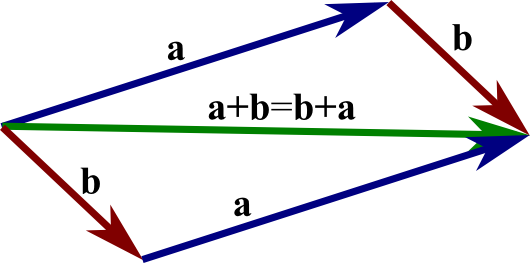
\includegraphics[width=0.75\textwidth]{add-vectors.png}
    \end{figure}
\end{exercisebox}

\subsubsection*{Vector Subtraction}
\addcontentsline{toc}{subsubsection}{Vector Subtraction}

The difference \(\vv{v} - \vv{w}\) is defined as \(\vv{v} + (-\vv{w})\), where \(-\vv{w}\) is the vector with the same magnitude as \(\vv{w}\) but opposite direction.

\begin{exercisebox}
    \textbf{Vector Subtraction} \\
    Given vectors \(\vv{v}\) and \(\vv{w}\), sketch \(\vv{v} - \vv{w}\).
\end{exercisebox}

\subsection*{Vector Components}
\addcontentsline{toc}{subsection}{Vector Components}

A vector in standard position has its initial point at the origin \((0, 0)\). If the terminal point is \((x, y)\), the vector is written in \textbf{component form} as \(\vv{v} = \langle x, y \rangle\). The scalars \(x\) and \(y\) are called the \textbf{components} of \(\vv{v}\).

\begin{exercisebox}
    \textbf{Expressing Vectors in Component Form} \\
    Express vector \(\vv{v}\) with initial point \((-3, 4)\) and terminal point \((1, 2)\) in component form.
\end{exercisebox}

\subsection*{Magnitude of a Vector}
\addcontentsline{toc}{subsection}{Magnitude of a Vector}

\begin{definitionbox}
    The magnitude of a vector \(\vv{v} = \langle x, y \rangle\) is its length, and is given by:
    \[
    \|\vv{v}\| = \sqrt{x^2 + y^2}.
    \]
\end{definitionbox}

\begin{exercisebox}
    Find the magnitude of the vector \(\vv{v} = \langle 3, -4 \rangle\).
\end{exercisebox}

\subsection*{Properties of Vector Operations}
\addcontentsline{toc}{subsection}{Properties of Vector Operations}

\begin{theorembox}
    Let \(\vv{u}\), \(\vv{v}\), and \(\vv{w}\) be vectors, and let \(k\) and \(c\) be scalars. Then:
    \begin{enumerate}
        \item \(\vv{u} + \vv{v} = \vv{v} + \vv{u}\) \quad (Commutative Property)
        \item \((\vv{u} + \vv{v}) + \vv{w} = \vv{u} + (\vv{v} + \vv{w})\) \quad (Associative Property)
        \item \(k(c\vv{v}) = (kc)\vv{v}\) \quad (Associativity of Scalar Multiplication)
        \item \(k(\vv{u} + \vv{v}) = k\vv{u} + k\vv{v}\) \quad (Distributive Property)
    \end{enumerate}
\end{theorembox}

\begin{proofbox}
    \textbf{Proof of Commutative Property:} \\
    Let \(\vv{u} = \langle u_1, u_2 \rangle\) and \(\vv{v} = \langle v_1, v_2 \rangle\). Then:
    \[
    \vv{u} + \vv{v} = \langle u_1 + v_1, u_2 + v_2 \rangle = \langle v_1 + u_1, v_2 + u_2 \rangle = \vv{v} + \vv{u}.
    \]
\end{proofbox}

\subsection*{Applications of Vectors}
\addcontentsline{toc}{subsection}{Applications of Vectors}

\begin{examplebox}
    \textbf{Real-Life Applications}
    \begin{itemize}
        \item A boat crossing a river experiences a force from its motor and a force from the river current. Both forces are vectors.
        \item A quarterback throwing a football applies a velocity vector to the ball, determining its speed and direction.
    \end{itemize}
\end{examplebox}

\subsection*{Learning Objectives}
\addcontentsline{toc}{subsection}{Learning Objectives}

By the end of this section, you should be able to:
\begin{itemize}
    \item Describe three-dimensional space mathematically.
    \item Locate points in space using coordinates.
    \item Write the distance formula in three dimensions.
    \item Write the equations for simple planes and spheres.
    \item Perform vector operations in \(\mathbb{R}^3\).
\end{itemize}

\subsection*{Introduction to Three-Dimensional Space}
\addcontentsline{toc}{subsection}{Introduction to Three-Dimensional Space}

\begin{definitionbox}
    \textbf{Definition:} The \textbf{three-dimensional rectangular coordinate system} consists of three perpendicular axes: the \(x\)-axis, the \(y\)-axis, and the \(z\)-axis, with an origin at the point of intersection \((0, 0, 0)\). This system is often denoted by \(\mathbb{R}^3\).
\end{definitionbox}

\begin{notebox}
    \textbf{Note:} The three-dimensional coordinate system follows the \textbf{right-hand rule}. If you align your right hand’s fingers with the positive \(x\)-axis and curl them toward the positive \(y\)-axis, your thumb points in the direction of the positive \(z\)-axis.
\end{notebox}

\subsection*{Locating Points in Space}
\addcontentsline{toc}{subsection}{Locating Points in Space}

\begin{definitionbox}
    \textbf{Definition:} A point in three-dimensional space is represented by coordinates \((x, y, z)\), where:
    \begin{itemize}
        \item \(x\) is the distance along the \(x\)-axis,
        \item \(y\) is the distance along the \(y\)-axis,
        \item \(z\) is the distance along the \(z\)-axis.
    \end{itemize}
\end{definitionbox}

\begin{examplebox}
    \textbf{Example 2.11: Locating Points in Space} \\
    Sketch the point \((1, -2, 3)\) in three-dimensional space.
\end{examplebox}

\begin{exercisebox}
    \textbf{Checkpoint 2.11:} \\
    Sketch the point \((-2, 3, -1)\) in three-dimensional space.
\end{exercisebox}

\subsection*{Coordinate Planes in \(\mathbb{R}^3\)}
\addcontentsline{toc}{subsection}{Coordinate Planes in \(\mathbb{R}^3\)}

\begin{definitionbox}
    \textbf{Definition:} The three coordinate planes in \(\mathbb{R}^3\) are:
    \begin{itemize}
        \item The \(xy\)-plane: \(\{(x, y, 0) \mid x, y \in \mathbb{R}\}\),
        \item The \(xz\)-plane: \(\{(x, 0, z) \mid x, z \in \mathbb{R}\}\),
        \item The \(yz\)-plane: \(\{(0, y, z) \mid y, z \in \mathbb{R}\}\).
    \end{itemize}
\end{definitionbox}

\begin{notebox}
    \textbf{Note:} The coordinate planes divide space into eight regions called \textbf{octants}. The first octant is where \(x > 0\), \(y > 0\), and \(z > 0\).
\end{notebox}

\subsection*{Distance Formula in Three Dimensions}
\addcontentsline{toc}{subsection}{Distance Formula in Three Dimensions}

\begin{theorembox}
    \textbf{Theorem 2.2: Distance Between Two Points in Space} \\
    The distance \(d\) between points \(P_1 = (x_1, y_1, z_1)\) and \(P_2 = (x_2, y_2, z_2)\) is given by:
    \[
    d = \sqrt{(x_2 - x_1)^2 + (y_2 - y_1)^2 + (z_2 - z_1)^2}.
    \]
\end{theorembox}

\begin{examplebox}
    \textbf{Example 2.12: Distance in Space} \\
    Find the distance between points \(P_1 = (3, -1, 5)\) and \(P_2 = (2, 1, -1)\).
\end{examplebox}

\begin{exercisebox}
    \textbf{Checkpoint 2.12:} \\
    Find the distance between points \(P_1 = (1, -5, 4)\) and \(P_2 = (4, -1, -1)\).
\end{exercisebox}

\subsection*{Equations of Planes}
\addcontentsline{toc}{subsection}{Equations of Planes}

\begin{definitionbox}
    \textbf{Definition:} A plane parallel to one of the coordinate planes can be described by:
    \begin{itemize}
        \item \(z = c\) for a plane parallel to the \(xy\)-plane,
        \item \(y = b\) for a plane parallel to the \(xz\)-plane,
        \item \(x = a\) for a plane parallel to the \(yz\)-plane.
    \end{itemize}
\end{definitionbox}

\begin{examplebox}
    \textbf{Example 2.13: Writing Equations of Planes} \\
    \begin{itemize}
        \item Write an equation of the plane passing through point \((3, 11, 7)\) that is parallel to the \(yz\)-plane.
        \item Find an equation of the plane passing through points \((6, -2, 9)\), \((0, -2, 4)\), and \((1, -2, -3)\).
    \end{itemize}
\end{examplebox}

\begin{exercisebox}
    \textbf{Checkpoint 2.13:} \\
    Write an equation of the plane passing through point \((1, -6, -4)\) that is parallel to the \(xy\)-plane.
\end{exercisebox}

\subsection*{Equations of Spheres}
\addcontentsline{toc}{subsection}{Equations of Spheres}

\begin{definitionbox}
    \textbf{Definition:} A \textbf{sphere} is the set of all points in space equidistant from a fixed point, called the \textbf{center}. The distance from the center to any point on the sphere is called the \textbf{radius}.
\end{definitionbox}

\begin{theorembox}
    \textbf{Equation of a Sphere:} \\
    The sphere with center \((a, b, c)\) and radius \(r\) is given by:
    \[
    (x - a)^2 + (y - b)^2 + (z - c)^2 = r^2.
    \]
\end{theorembox}

\begin{examplebox}
    \textbf{Example 2.14: Finding an Equation of a Sphere} \\
    Find the standard equation of the sphere with center \((10, 7, 4)\) and passing through point \((-1, 3, -2)\).
\end{examplebox}

\begin{exercisebox}
    \textbf{Checkpoint 2.14:} \\
    Find the standard equation of the sphere with center \((-2, 4, -5)\) and passing through point \((4, 4, -1)\).
\end{exercisebox}

\begin{examplebox}
    \textbf{Example 2.15: Finding the Equation of a Sphere} \\
    Let \(P = (-5, 2, 3)\) and \(Q = (3, 4, -1)\), and suppose line segment \(PQ\) forms the diameter of a sphere. Find the equation of the sphere.
\end{examplebox}

\begin{exercisebox}
    \textbf{Checkpoint 2.15:} \\
    Find the equation of the sphere with diameter \(PQ\), where \(P = (2, -1, -3)\) and \(Q = (-2, 5, -1)\).
\end{exercisebox}

\subsection*{Graphing Equations in Three Dimensions}
\addcontentsline{toc}{subsection}{Graphing Equations in Three Dimensions}

\begin{examplebox}
    \textbf{Example 2.16: Graphing Other Equations} \\
    Describe the set of points that satisfies \((x - 4)(z - 2) = 0\), and graph the set.
\end{examplebox}

\begin{exercisebox}
    \textbf{Checkpoint 2.16:} \\
    Describe the set of points that satisfies \((y + 2)(z - 3) = 0\), and graph the set.
\end{exercisebox}

\begin{examplebox}
    \textbf{Example 2.17: Graphing Other Equations} \\
    Describe the set of points in three-dimensional space that satisfies \((x - 2)^2 + (y - 1)^2 = 4\), and graph the set.
\end{examplebox}

\begin{exercisebox}
    \textbf{Checkpoint 2.17:} \\
    Describe the set of points in three-dimensional space that satisfies \(x^2 + (z - 2)^2 = 16\), and graph the surface.
\end{exercisebox}

\textbf{self-note: add the rest from deepseek alexandermenginquiries@gmail.com account}

\cleardoublepage
\phantomsection
\begin{titlepage}
    \null % Ensures proper alignment with vfill
    \vfill
    \begin{center}
        {\Huge \textbf{Let’s Get Started}} \\[20pt]
        \rule{\textwidth}{0.5mm} \\[15pt]
        {\Large \textit{Time to dive into the lecture notes.}} \\[15pt]
        \rule{\textwidth}{0.5mm} \\[15pt]
        \textbf{Grab your pen or pencil, and let’s break this down step by step.}
    \end{center}
    \vfill
\end{titlepage}

\addcontentsline{toc}{section}{Lecture Content}

\normalsize

\setcounter{page}{1}

\end{document}
